\documentclass[border=0.5cm]{standalone}
 
% Package
\usepackage[RPvoltages]{circuitikz}
 
\begin{document}
 
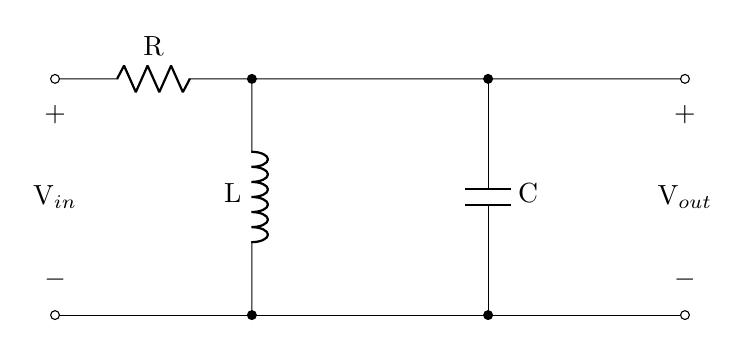
\begin{tikzpicture}[american]
 
% Components size
\ctikzset{
    resistors/scale=0.8,
    capacitors/scale=0.7,
    inductors/coils=6
}

 
% Circuit code
\draw (0,3) to[R,l=R,o-] ++(2.5,0) coordinate(a1)
    to[short] ++(3,0) coordinate(a2)
    to[short,-o] ++ (2.5,0);
 
\draw (0,0) to[short,o-] ++(2.5,0) coordinate(a3)
    to[short] ++(3,0) coordinate(a4)
    to[short,-o] ++ (2.5,0);
 
\draw (a1) to[inductor,l_=L,*-*] (a3);
\draw (a2) to[C,l=C,*-*] (a4);
 
% Labels
\draw (0,3) to[open,v=V$_{in}$] ++(0,-3);
\draw (8,3) to[open,v=V$_{out}$] ++(0,-3);
 
\end{tikzpicture}
 
\end{document}